\section*{Supplemental Figures}

% k-mer distribution of the raw hi-fi reads
\begin{figure}[ht]
    \centering
    \captionsetup{width=0.95\linewidth}
    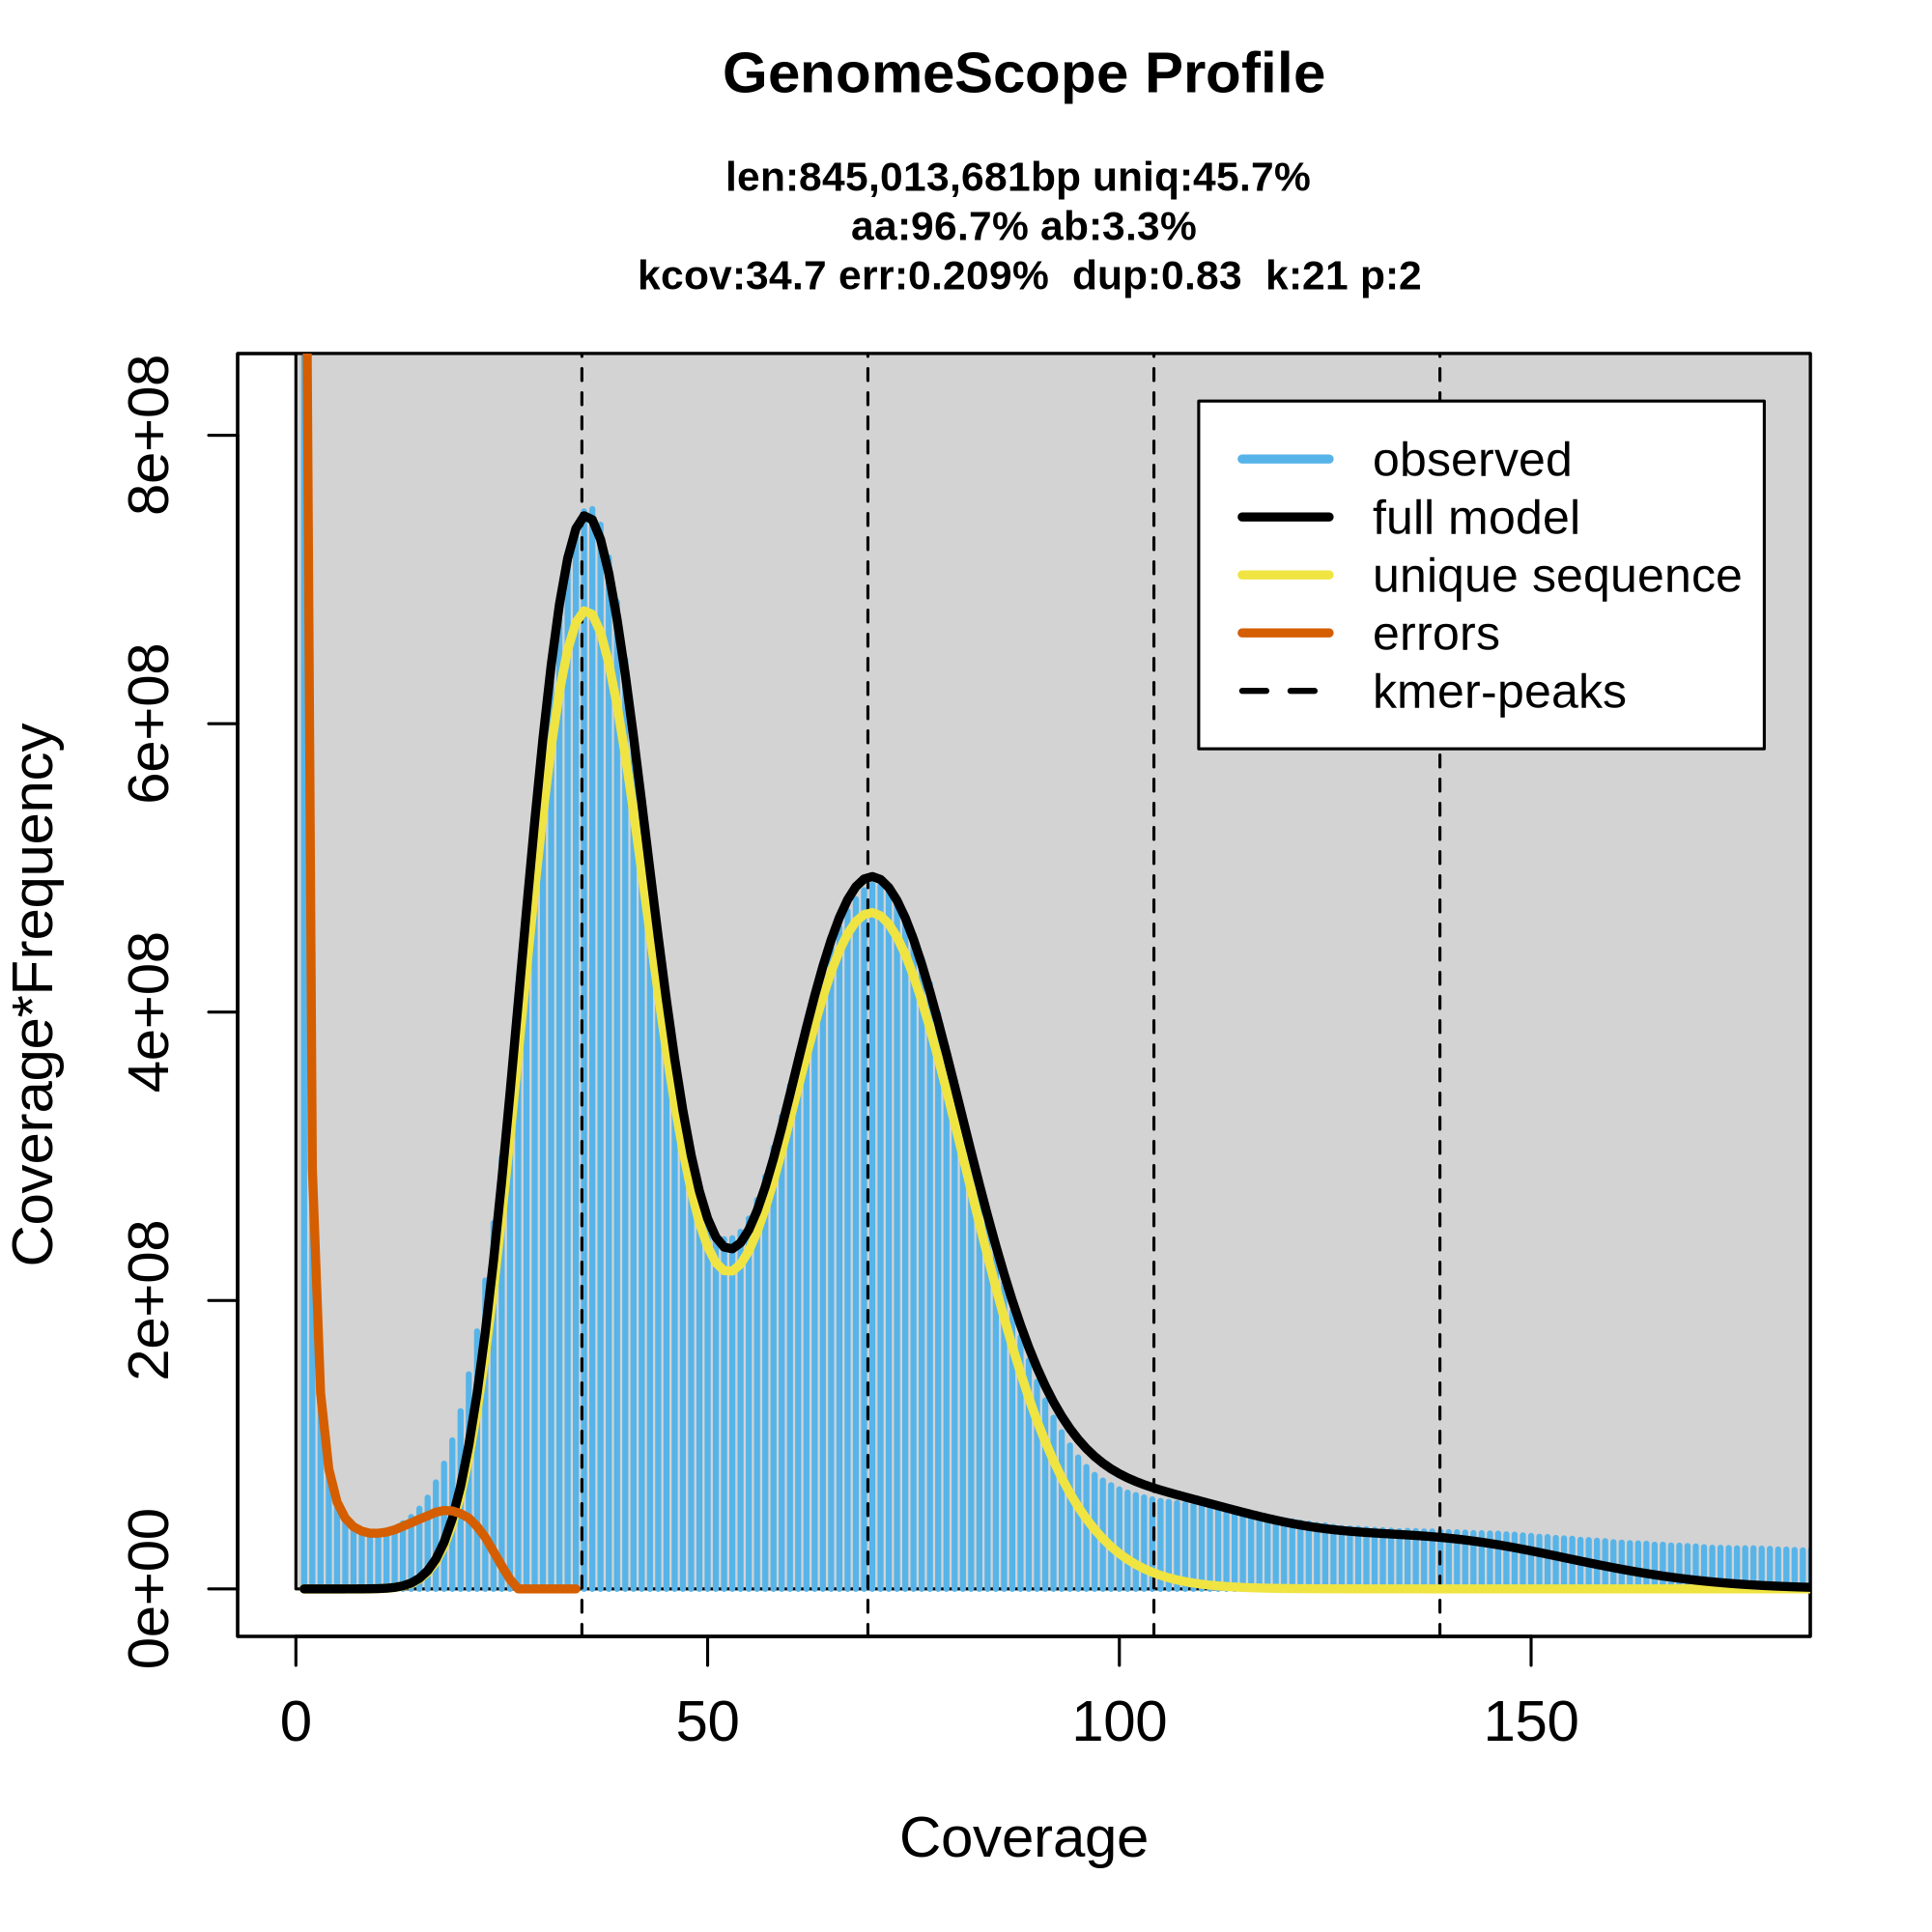
\includegraphics[width=0.8\textwidth]{figures/sups_kmers.png}
    \supfigurecaption{\textbf{\textsc{GenomeScope} profile of the raw PacBio HiFi
        data.} Distribution of 21-mers shows an estimated genome size of
        845.01 Mbp and a heterozygosity of 3.3\% in the \bgla{}
        reference assembly.}
    \label{fig:sup_kmers}
\end{figure}

% Hi-C contact map
\begin{figure}[ht]
    \centering
    \captionsetup{width=0.95\linewidth}
    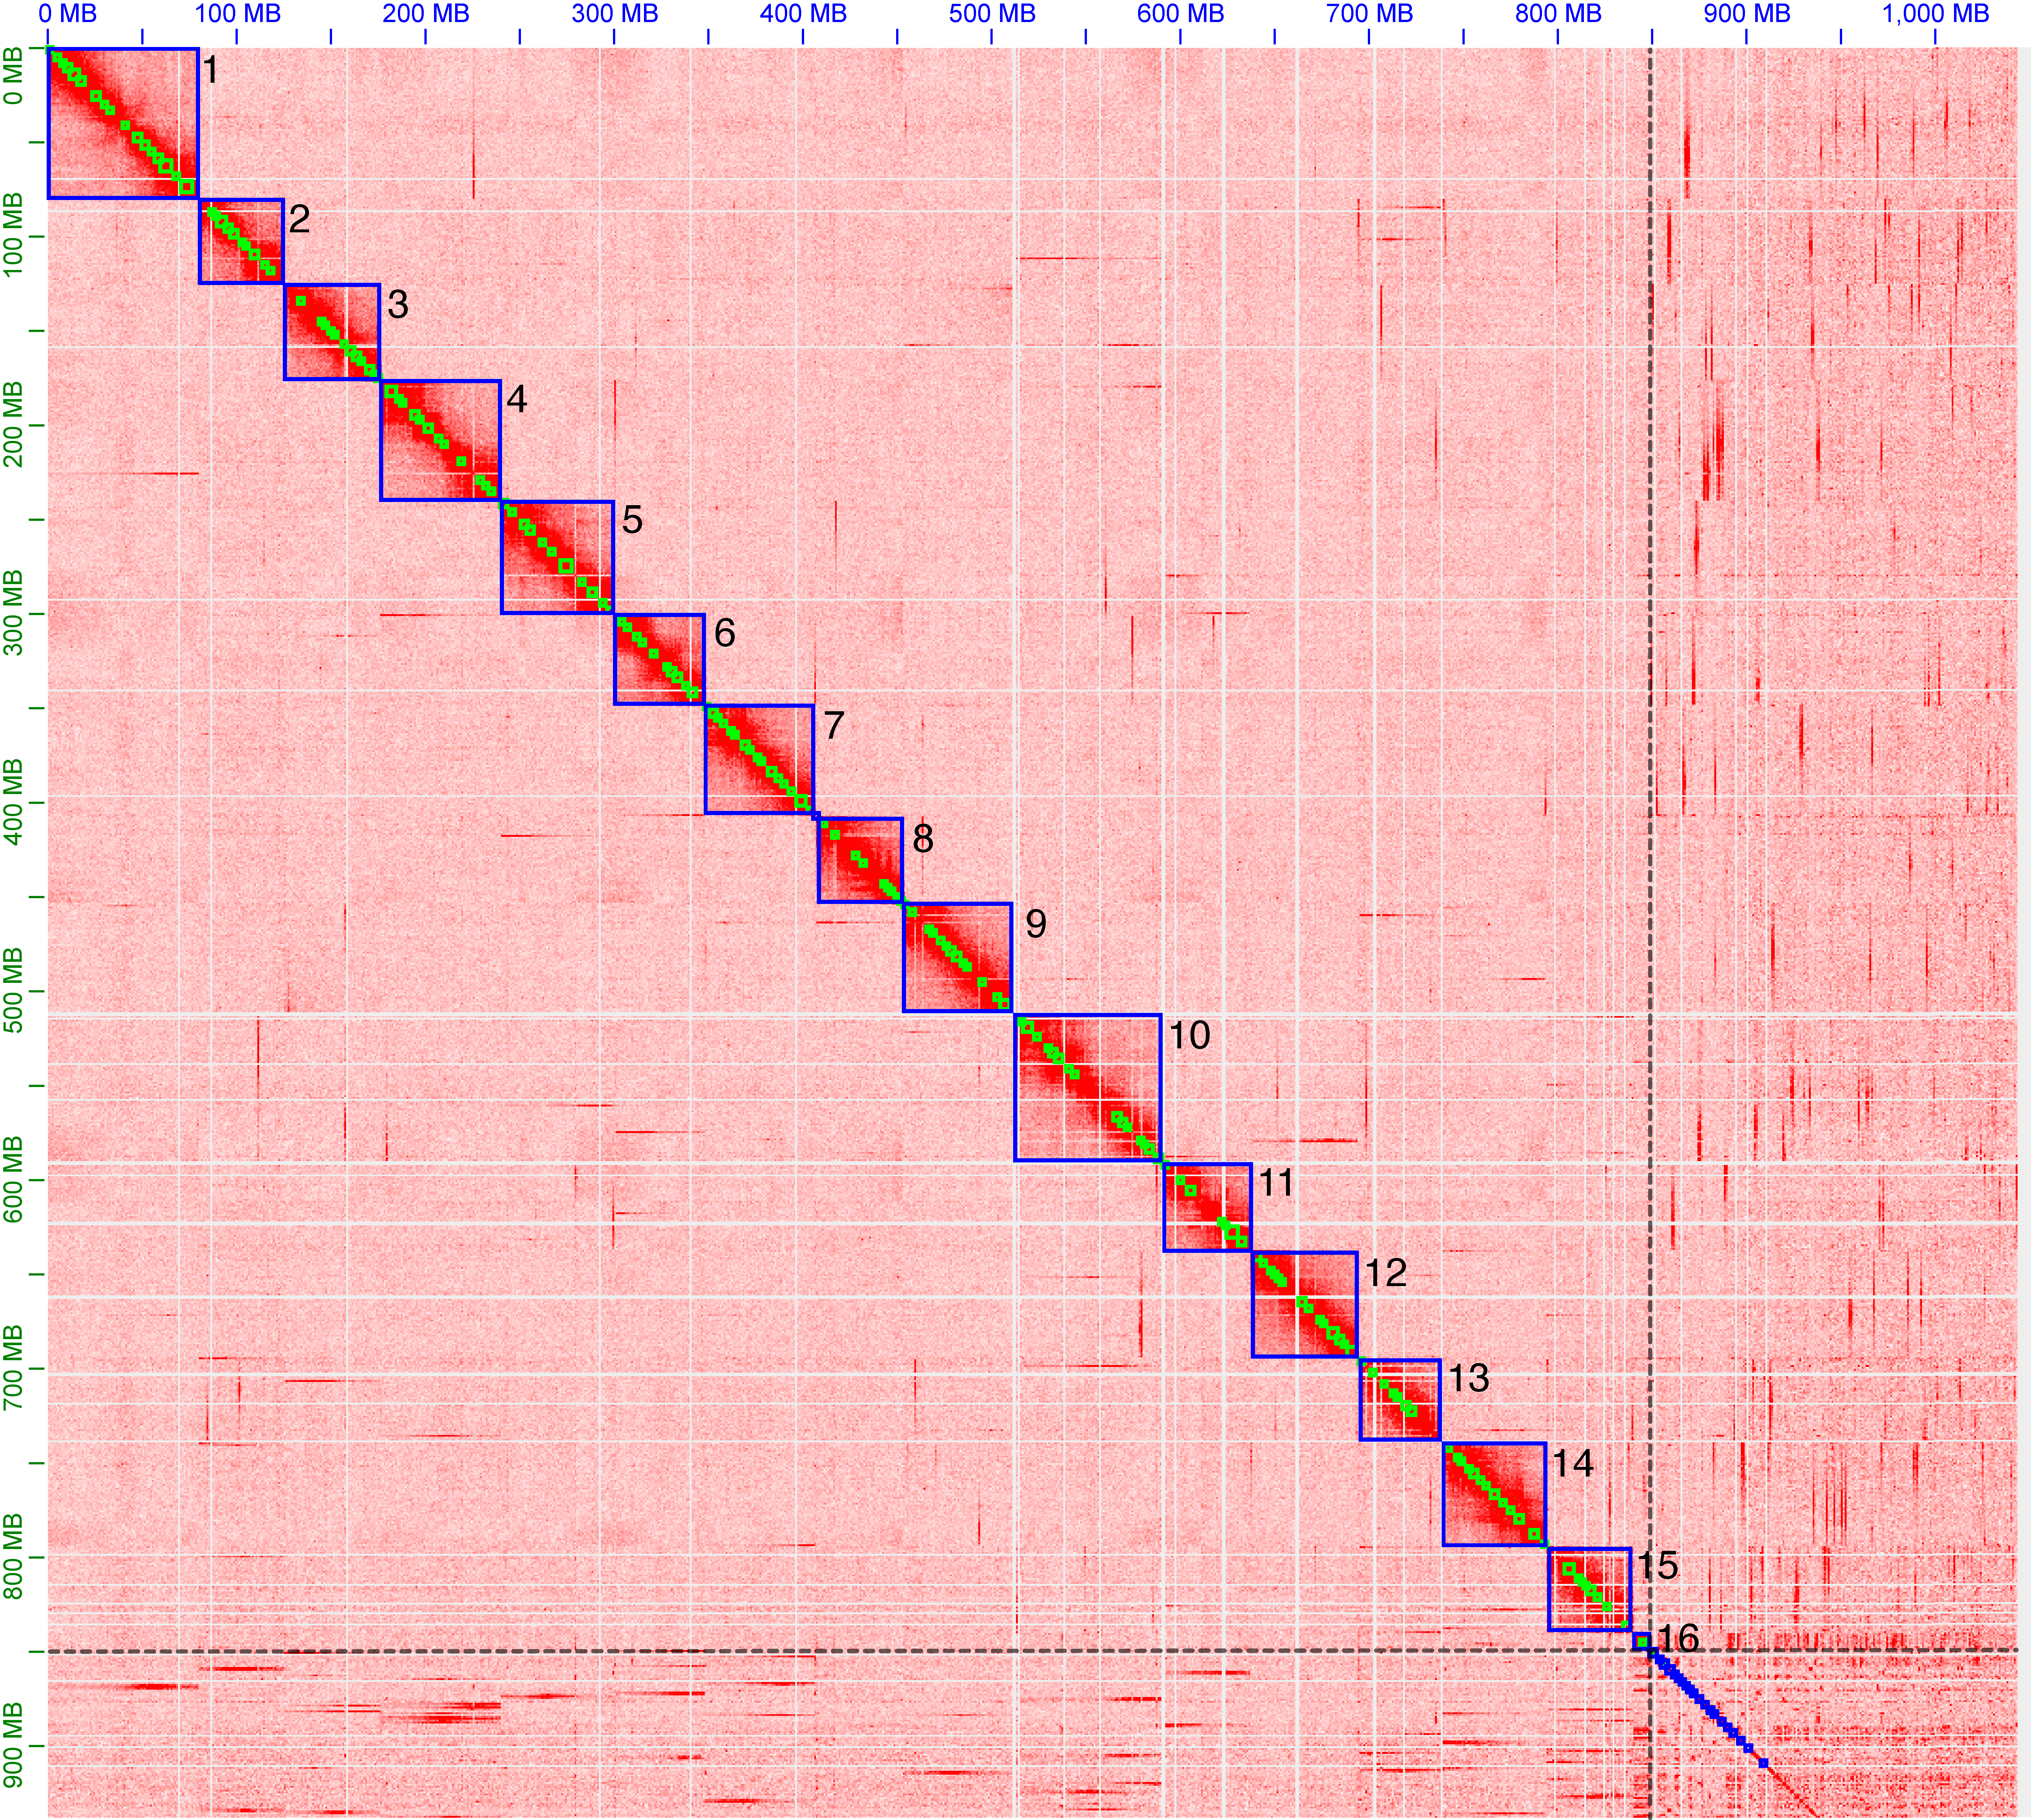
\includegraphics[width=1.0\textwidth]{figures/sups_hic.pdf}
    \supfigurecaption{\textbf{Hi-C contact map of the \balgla{} assembly.}
        The contact map shows the assembly following manual curation in
        \textsc{Juicebox}. The numbers (1--16) denote the 16 chromosome-level
        scaffolds. The dashed lines show the boundary between these 16
        chromosome-level scaffolds and the unplaced contigs. Note that this
        numbering does not reflect the final ID of the assembled sequences.
        IDs were re-assigned following additional curation and sorting of the
        sequences.}
    \label{fig:sup_hic}
\end{figure}

% dN/dS
\begin{figure}[ht]
    \centering
    \captionsetup{width=0.95\linewidth}
    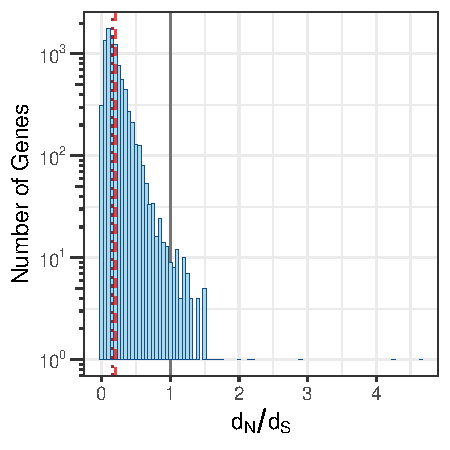
\includegraphics[width=0.7\textwidth]{figures/dnds.pdf}
    \supfigurecaption{\textbf{Distribution of the pairwise rate of non-synonymous
        to synonymous substitutions (\dnds{}).}
        The distribution is calculated across 9{,}082 single-copy orthologs
        identified between \balgla{} and \textit{Balanus
        crenatus}. The solid gray line marks the boundary between genes under
        positive selection (\dnds{} $>$ 1) and genes under purifying selection
        (\dnds{} $<$ 1). The dashed and dotted lines show the mean (0.206) and
        median (0.158) \dnds{}, both showing that on average \bgla{} coding
        sequences are evolving under a regime of purifying selection.}
    \label{fig:sup_dnds}
\end{figure}

% Direction of selection.
\begin{figure}[ht]
    \centering
    \captionsetup{width=0.95\linewidth}
    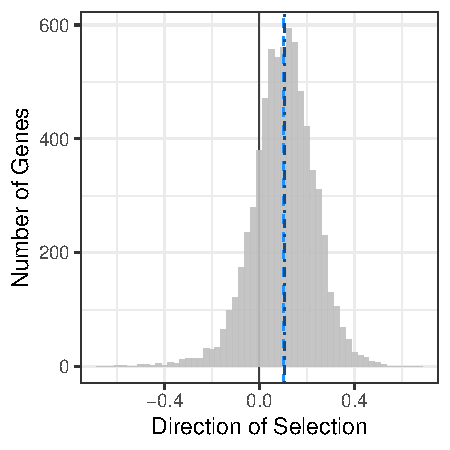
\includegraphics[width=0.7\textwidth]{figures/sups_mkt_dos.pdf}
    \supfigurecaption{\textbf{Distribution of per-gene direction of selection values.}
        The distribution shows Direction of Selection (DoS) calculated across 7{,}056
        single-copy orthologs identified between \balgla{} and
        \textit{Balanus crenatus}. The solid black line at zero marks the boundary
        between genes evolving under a regime of positive selection (DoS $>0$) and
        genes exhibiting an excess of slightly deleterious non-synonymous polymorphism
        (DoS $<0$). The light blue dashed line shows the mean DoS (0.103), while
        the dark blue dotted line shows the median DoS (0.109).
        This distribution shows that, on average, coding sequences in \bgla{} appear
        to be evolving under positive selection.}
    \label{fig:sup_dos}
\end{figure}

% Extended GO terms.
\begin{figure}[ht]
    \centering
    \captionsetup{width=0.95\linewidth}
    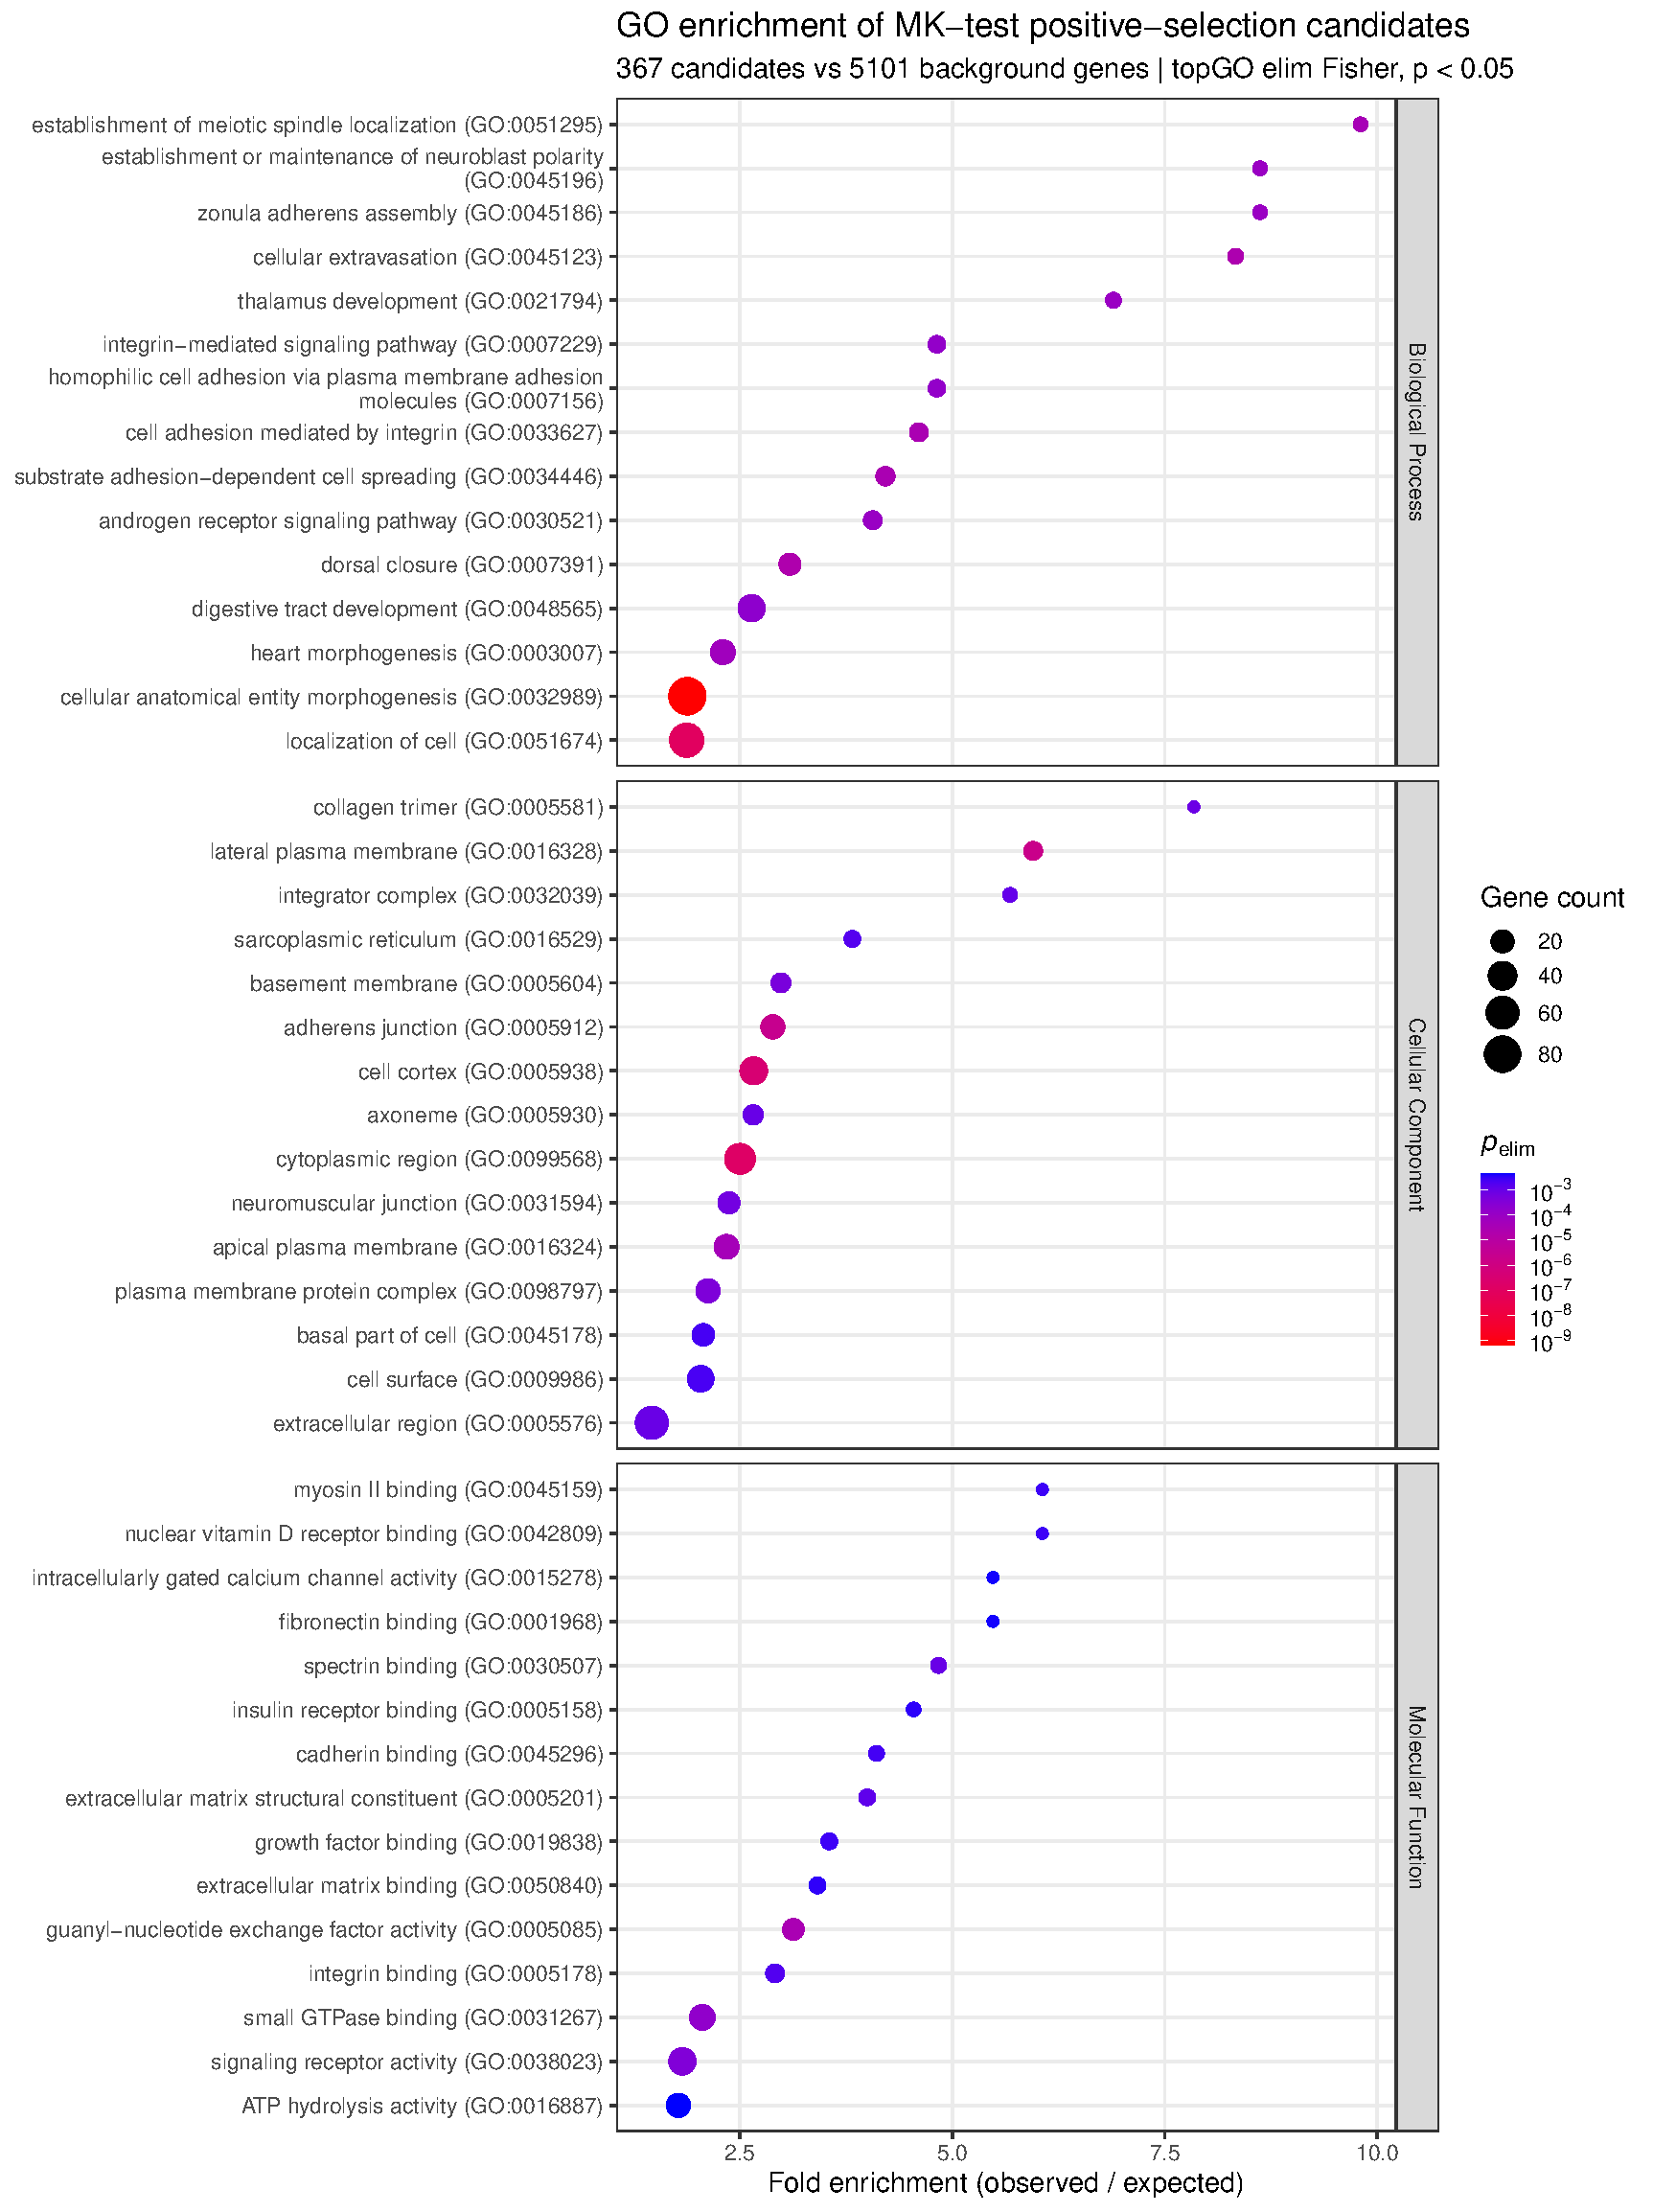
\includegraphics[width=0.925\textwidth]{figures/sups_go_extended.pdf}
    \supfigurecaption{\textbf{Significant GO term enrichment among the candidates
        under positive selection in the McDonald-Kreitman test.}
        Enrichment for the 367 candidates under selection with annotated GO terms.
        $p_\text{elim}$ denotes the $p$-value calculated from \textsc{topGO}'s
        \texttt{elim} algorithm.
        Top, middle, and bottom panels show the top 15 most enriched terms across
        the three GO categories: biological processes, cellular component, and
        molecular function.
        }
    \label{fig:sup_go}
\end{figure}

% Coding GC, GC3s, and GC4d
\begin{figure}[ht]
    \centering
    \captionsetup{width=0.95\linewidth}
    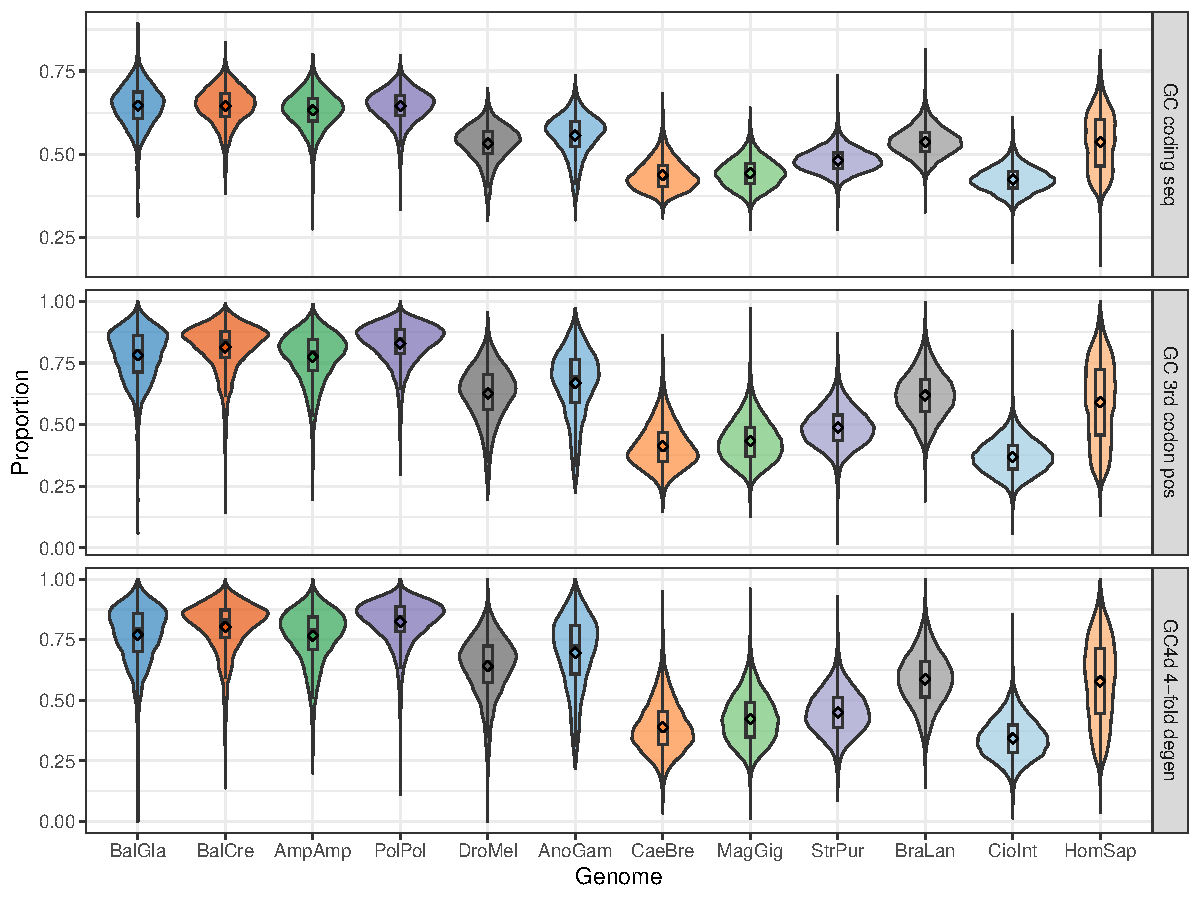
\includegraphics[width=1.0\textwidth]{figures/sups_coding_gc.pdf}
    \supfigurecaption{\textbf{Distribution of coding GC proportions across metazoan
        genomes.}
        Top, middle, and bottom panels show the GC proportions coding sequence-wide,
        at 3rd codon positions (GC3s), and at 4-fold degerate sites (GC4d),
        respectively.
        Distribution are shown across 12 metazoan genomes, including four barnacles:
        \bgla{} (\texttt{BalGla}), \textit{B. crenatus} (\texttt{BalCre}),
        \textit{A. amphitrite} (\texttt{AmpAmp}), and \textit{P. pollicipes}
        (\texttt{PolPol}).
        See Table~\ref{tab:sup_enc_summary} for additional description of the
        genomes.}
    \label{fig:sup_coding_gc}
\end{figure}

% ENC vs GC3s
\begin{figure}[ht]
    \centering
    \captionsetup{width=0.95\linewidth}
    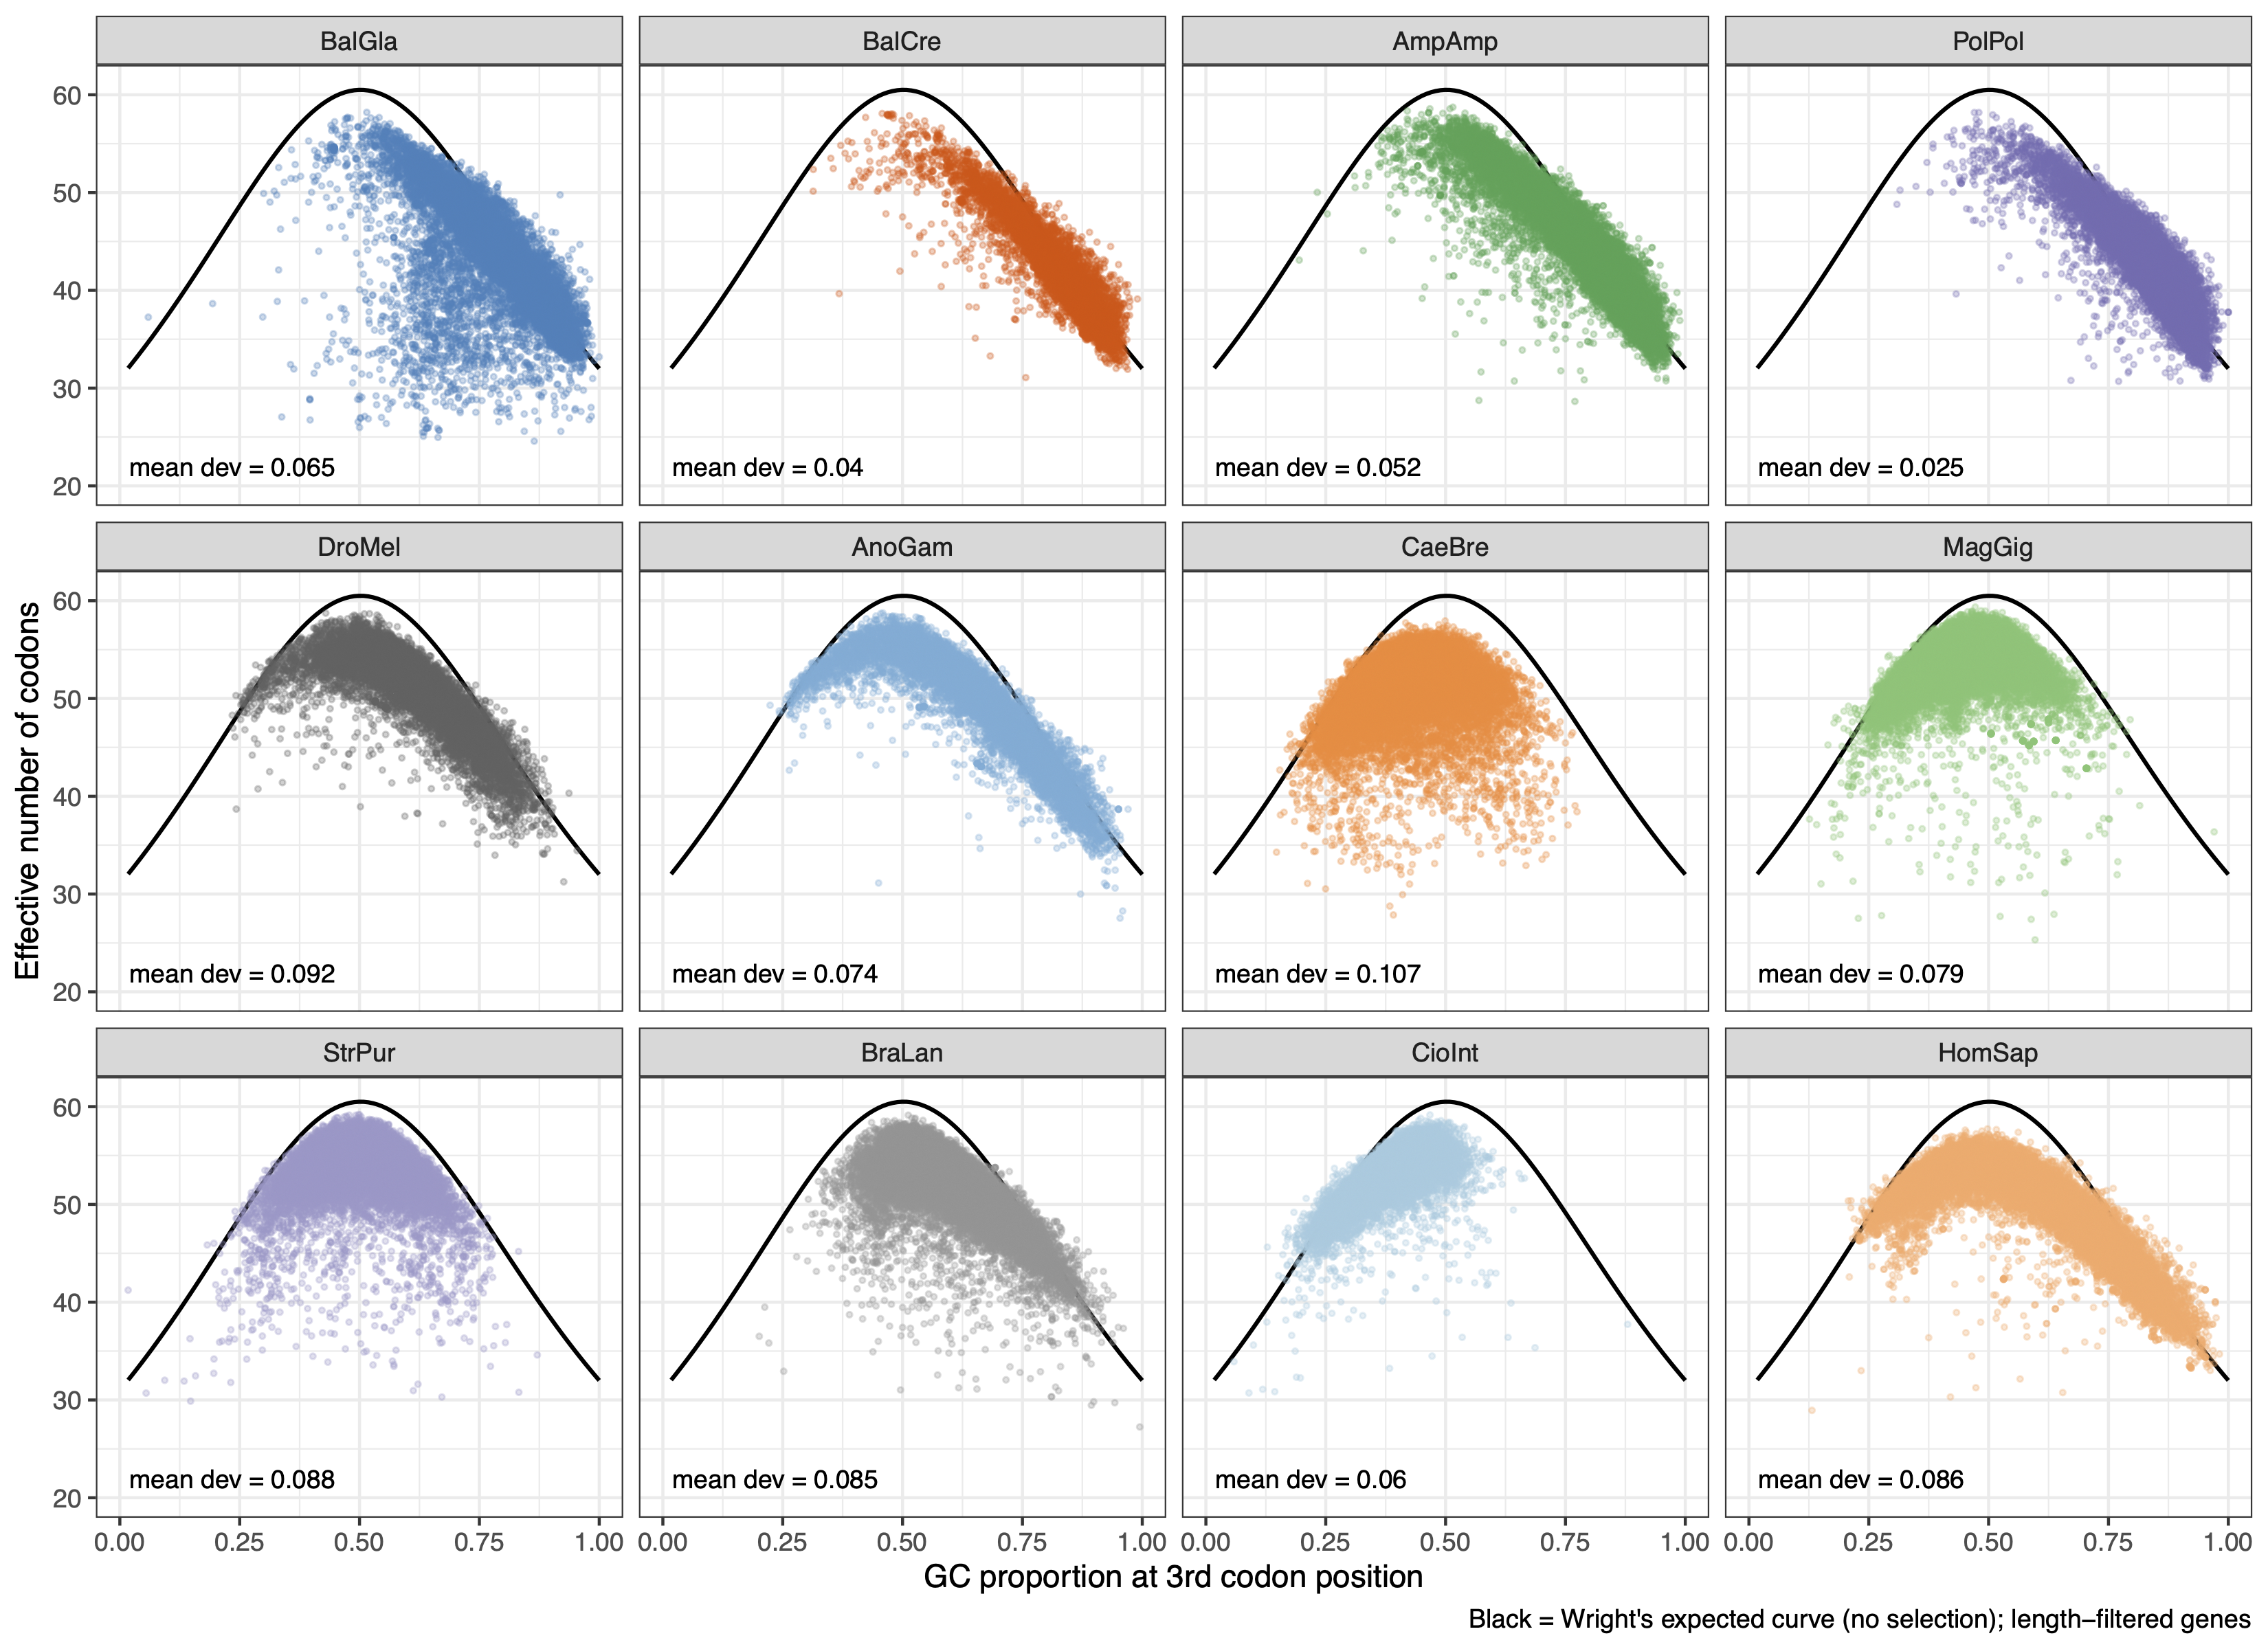
\includegraphics[width=1.0\textwidth]{figures/sups_enc_gc3s.png}
    \supfigurecaption{\textbf{Relationship between effective codons and GC content.}
        Nc-plots showing the relationship between GC proportion at 3rd codon positions
        (GC3s; X-axis) and the effective number of codons (ENC; Y-axis) for 12
        metazoan genomes.
        At each panel, each point represents a single gene.
        The black curve shows the expected relationship between GC3s and ENC, according
        to Wright's curve: \wrightenc{}, where $s$ denotes GC3s.
        The ``mean dev'' annotation shows the mean deviation in ENC from the theoretical
        expectation.
        Higher values show a larger proportion of genes showing a smaller than expected
        number of effective codons, a putative signature of translational selection.
        See Table~\ref{tab:sup_enc_summary} for additional description of the
        genomes.}
    \label{fig:sup_enc_gc3s}
\end{figure}

% Exp vs Obs ENC
\begin{figure}[ht]
    \centering
    \captionsetup{width=0.95\linewidth}
    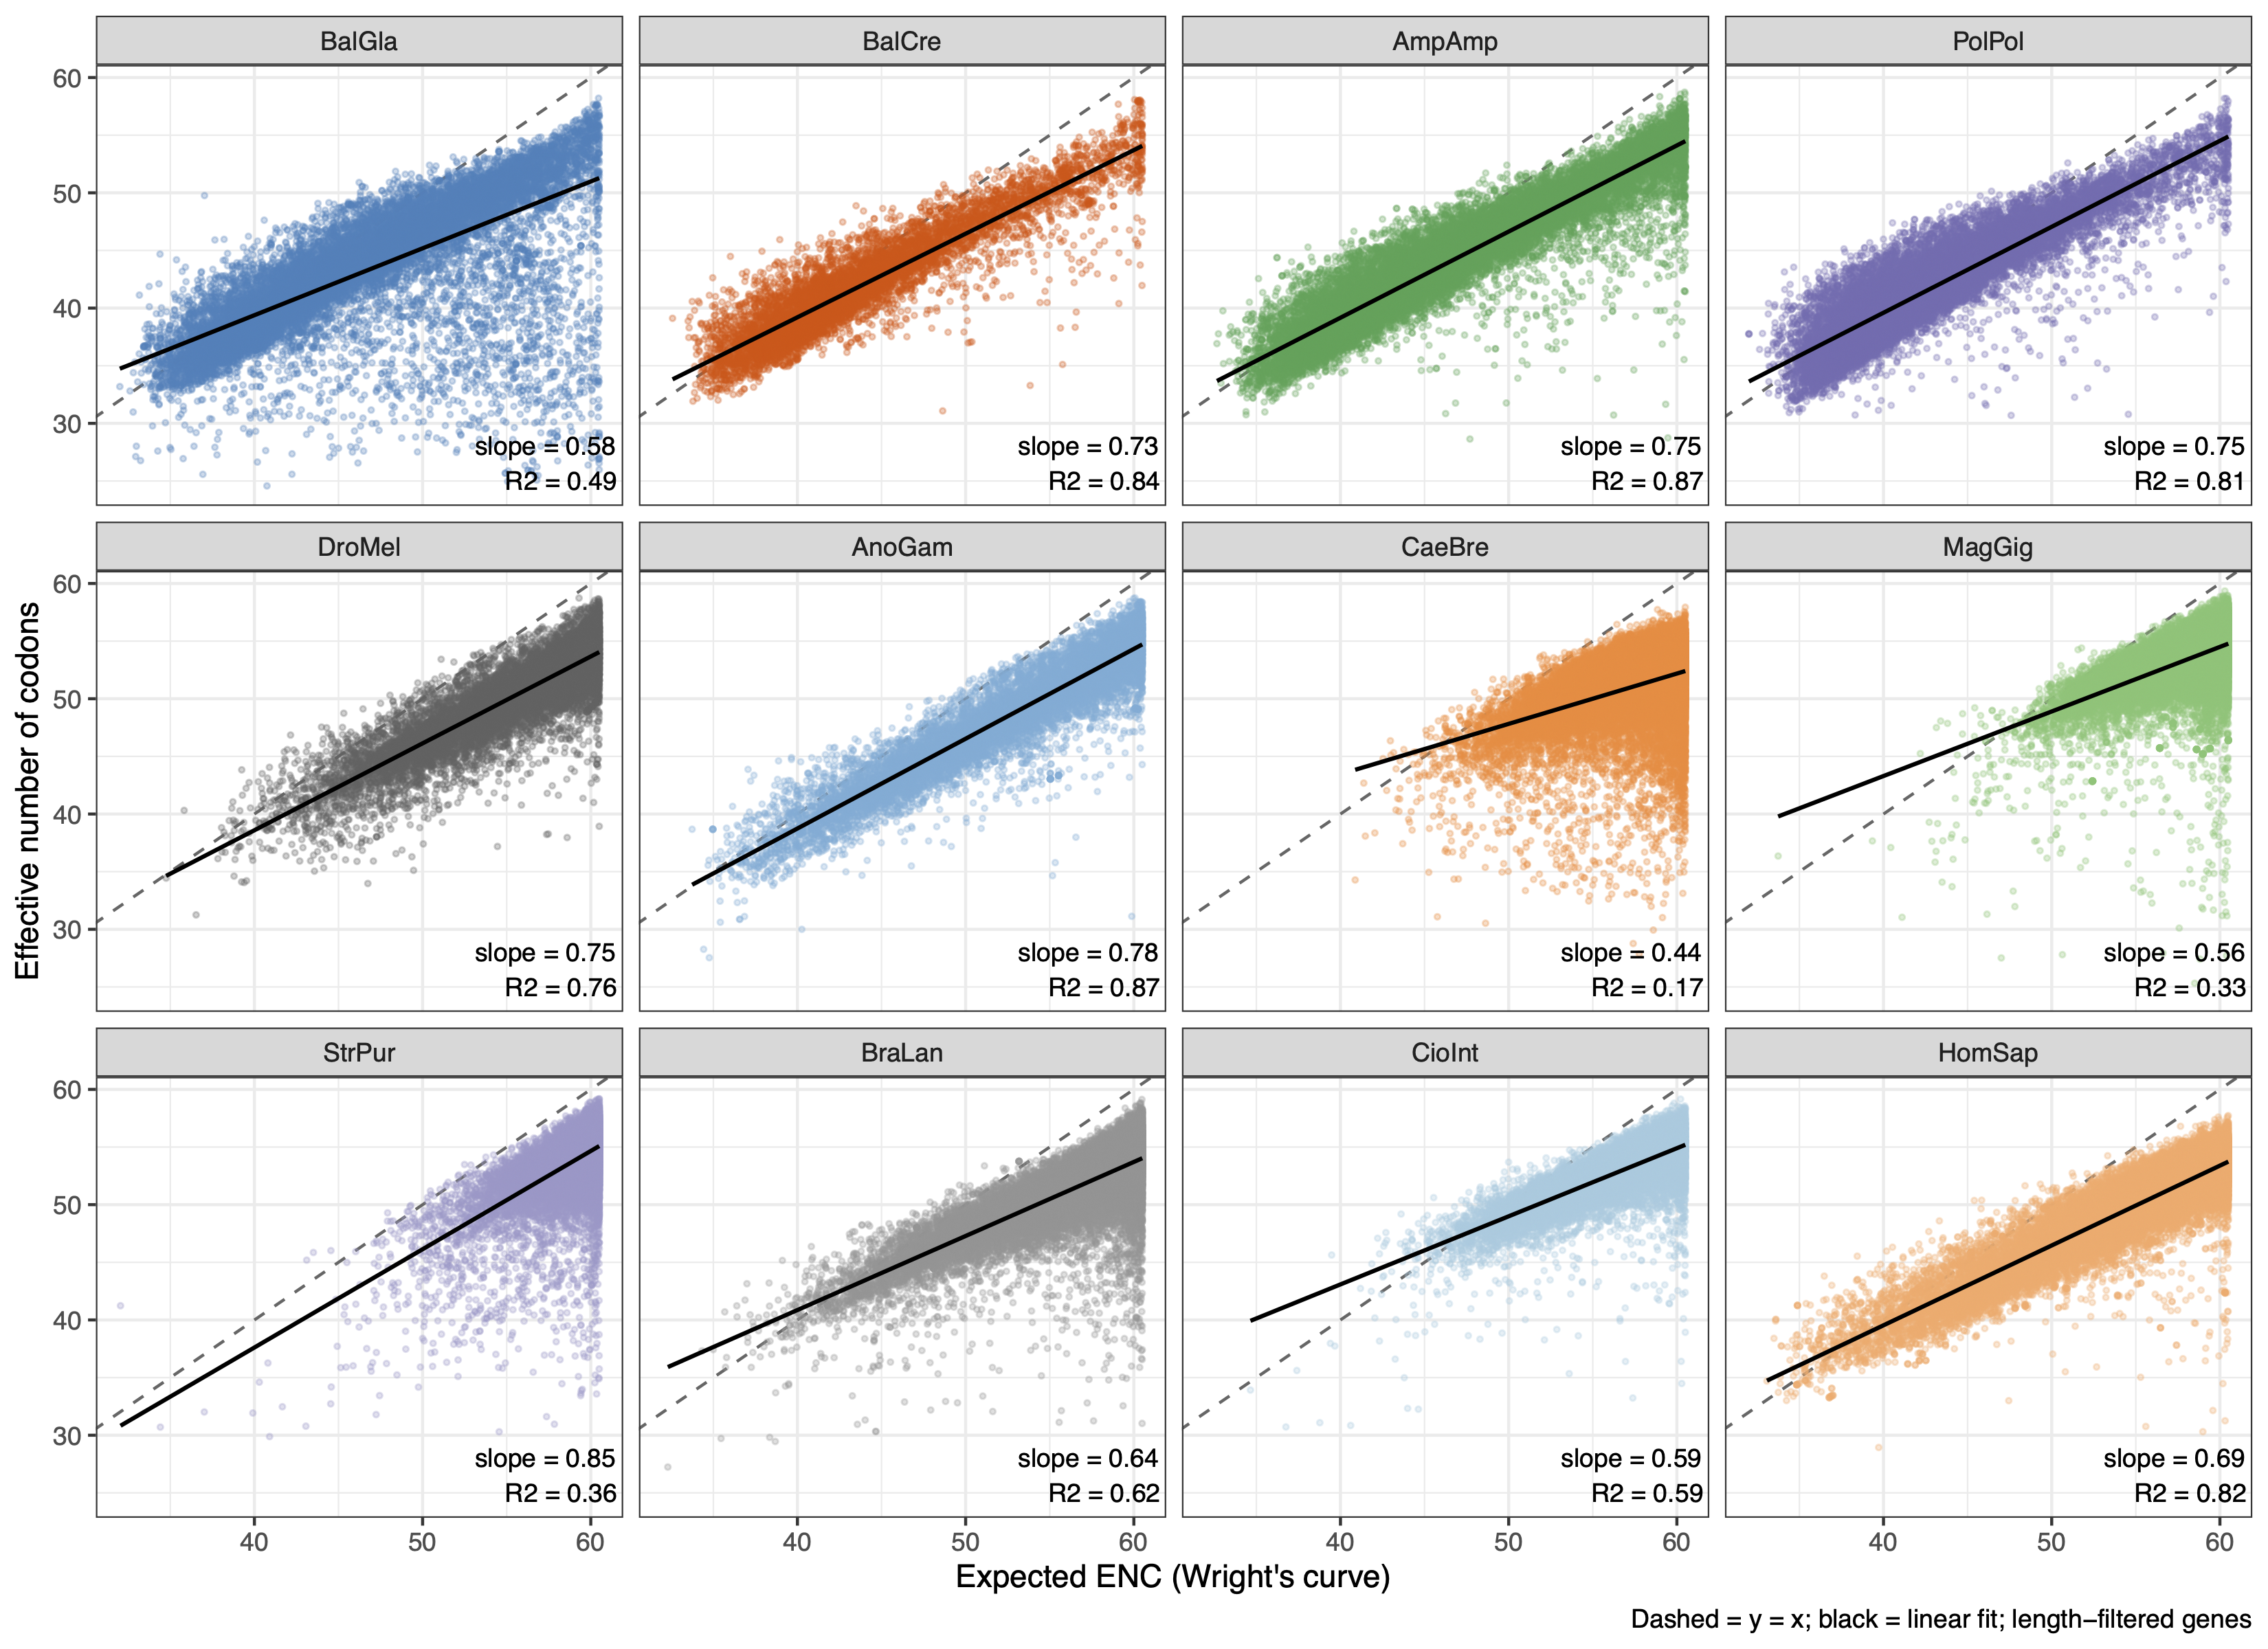
\includegraphics[width=1.0\textwidth]{figures/sups_enc_regression.png}
    \supfigurecaption{\textbf{Relationship between the expected and observed number of
        effective codons.}
        Plots show the observed effective number of codons (ENC; Y-axis) as a function
        of the expected ENC (X-axis), as defined by Wright's curve, for 12 metazoan
        genomes.
        At each panel, points represents single genes.
        Dashed line shows the one-to-one relationship, while the solid black line
        shows the linear regression.
        Annotations in the plot show the regression's slope and coefficient of
        determination ($\text{R}^2$).
        Small ($\ll1$) slopes and low $\text{R}^2$ show a reduction in the observed
        number of effective codons when compared to the theoretical expectation,
        a potential signature of translational selection.
        See Table~\ref{tab:sup_enc_summary} for additional description of the
        genomes.}
    \label{fig:sup_enc_reg}
\end{figure}

% Pi vs other species.
\begin{figure}[ht]
    \centering
    \captionsetup{width=0.95\linewidth}
    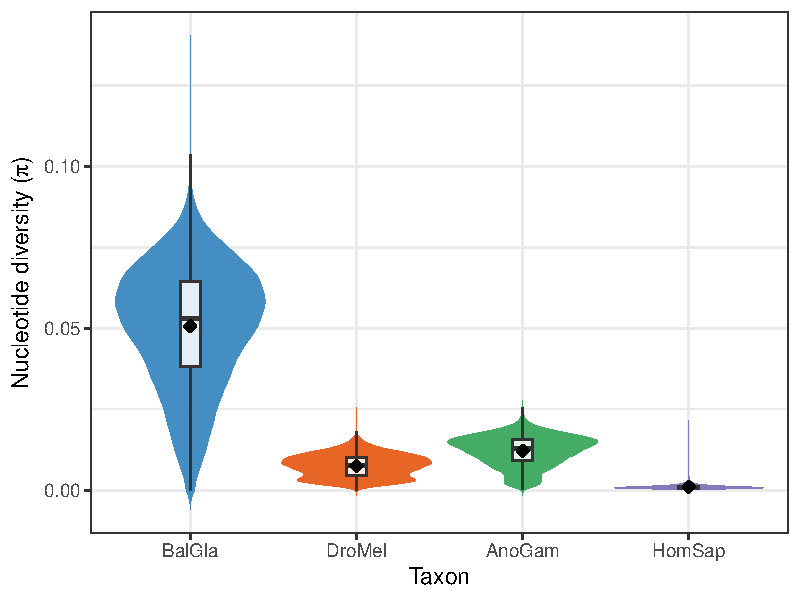
\includegraphics[width=0.9\textwidth]{figures/sups_pi_comparisons.pdf}
    \supfigurecaption{\textbf{Comparing nucleotide diversity ($\pi$) between
        barnacles and biological model systems.}
        Average $\pi$ in 10 kbp windows between the
        Oregon Pacific acorn barnacle (\balgla{}; \texttt{BalGla}),
        Sub-Saharan populations of the fruit fly (\textit{Drosophila melanogaster};
            \texttt{DroMel}),
        malaria mosquitoes from the Central African Republic (\textit{Anopheles
            gambiae}; \texttt{AnoGam}),
        and human populations of Yoruba ancestry (\textit{Homo sapiens}; \texttt{HomSap}).
        Consistent with the large \Ne{} expected for \bgla{}, this barnacle population
        exhibits an average nucleotide diversity (mean = 0.0506, median = 0.0532, standard
        deviation = 0.0188) an order of magnitude higher than \textit{Drosophila} (mean = 0.0076,
        median = 0.0078, standard deviation = 0.0035), $\approx4\times$ higher than
        \textit{An. gambiae} (mean = 0.0123, median = 0.0130, standard deviation = 0.0047), and
        $\approx48\times$ larger than diverse human cohorts (mean = 0.0011, median = $9.54\times10^{-4}$,
        standard deviation = $5.81\times10^{-4}$).}
    \label{fig:sup_pi_comp}
\end{figure}

% Pairwise correlation among different genomic feature and diversity metrics.
\begin{figure}[ht]
    \centering
    \captionsetup{width=0.95\linewidth}
    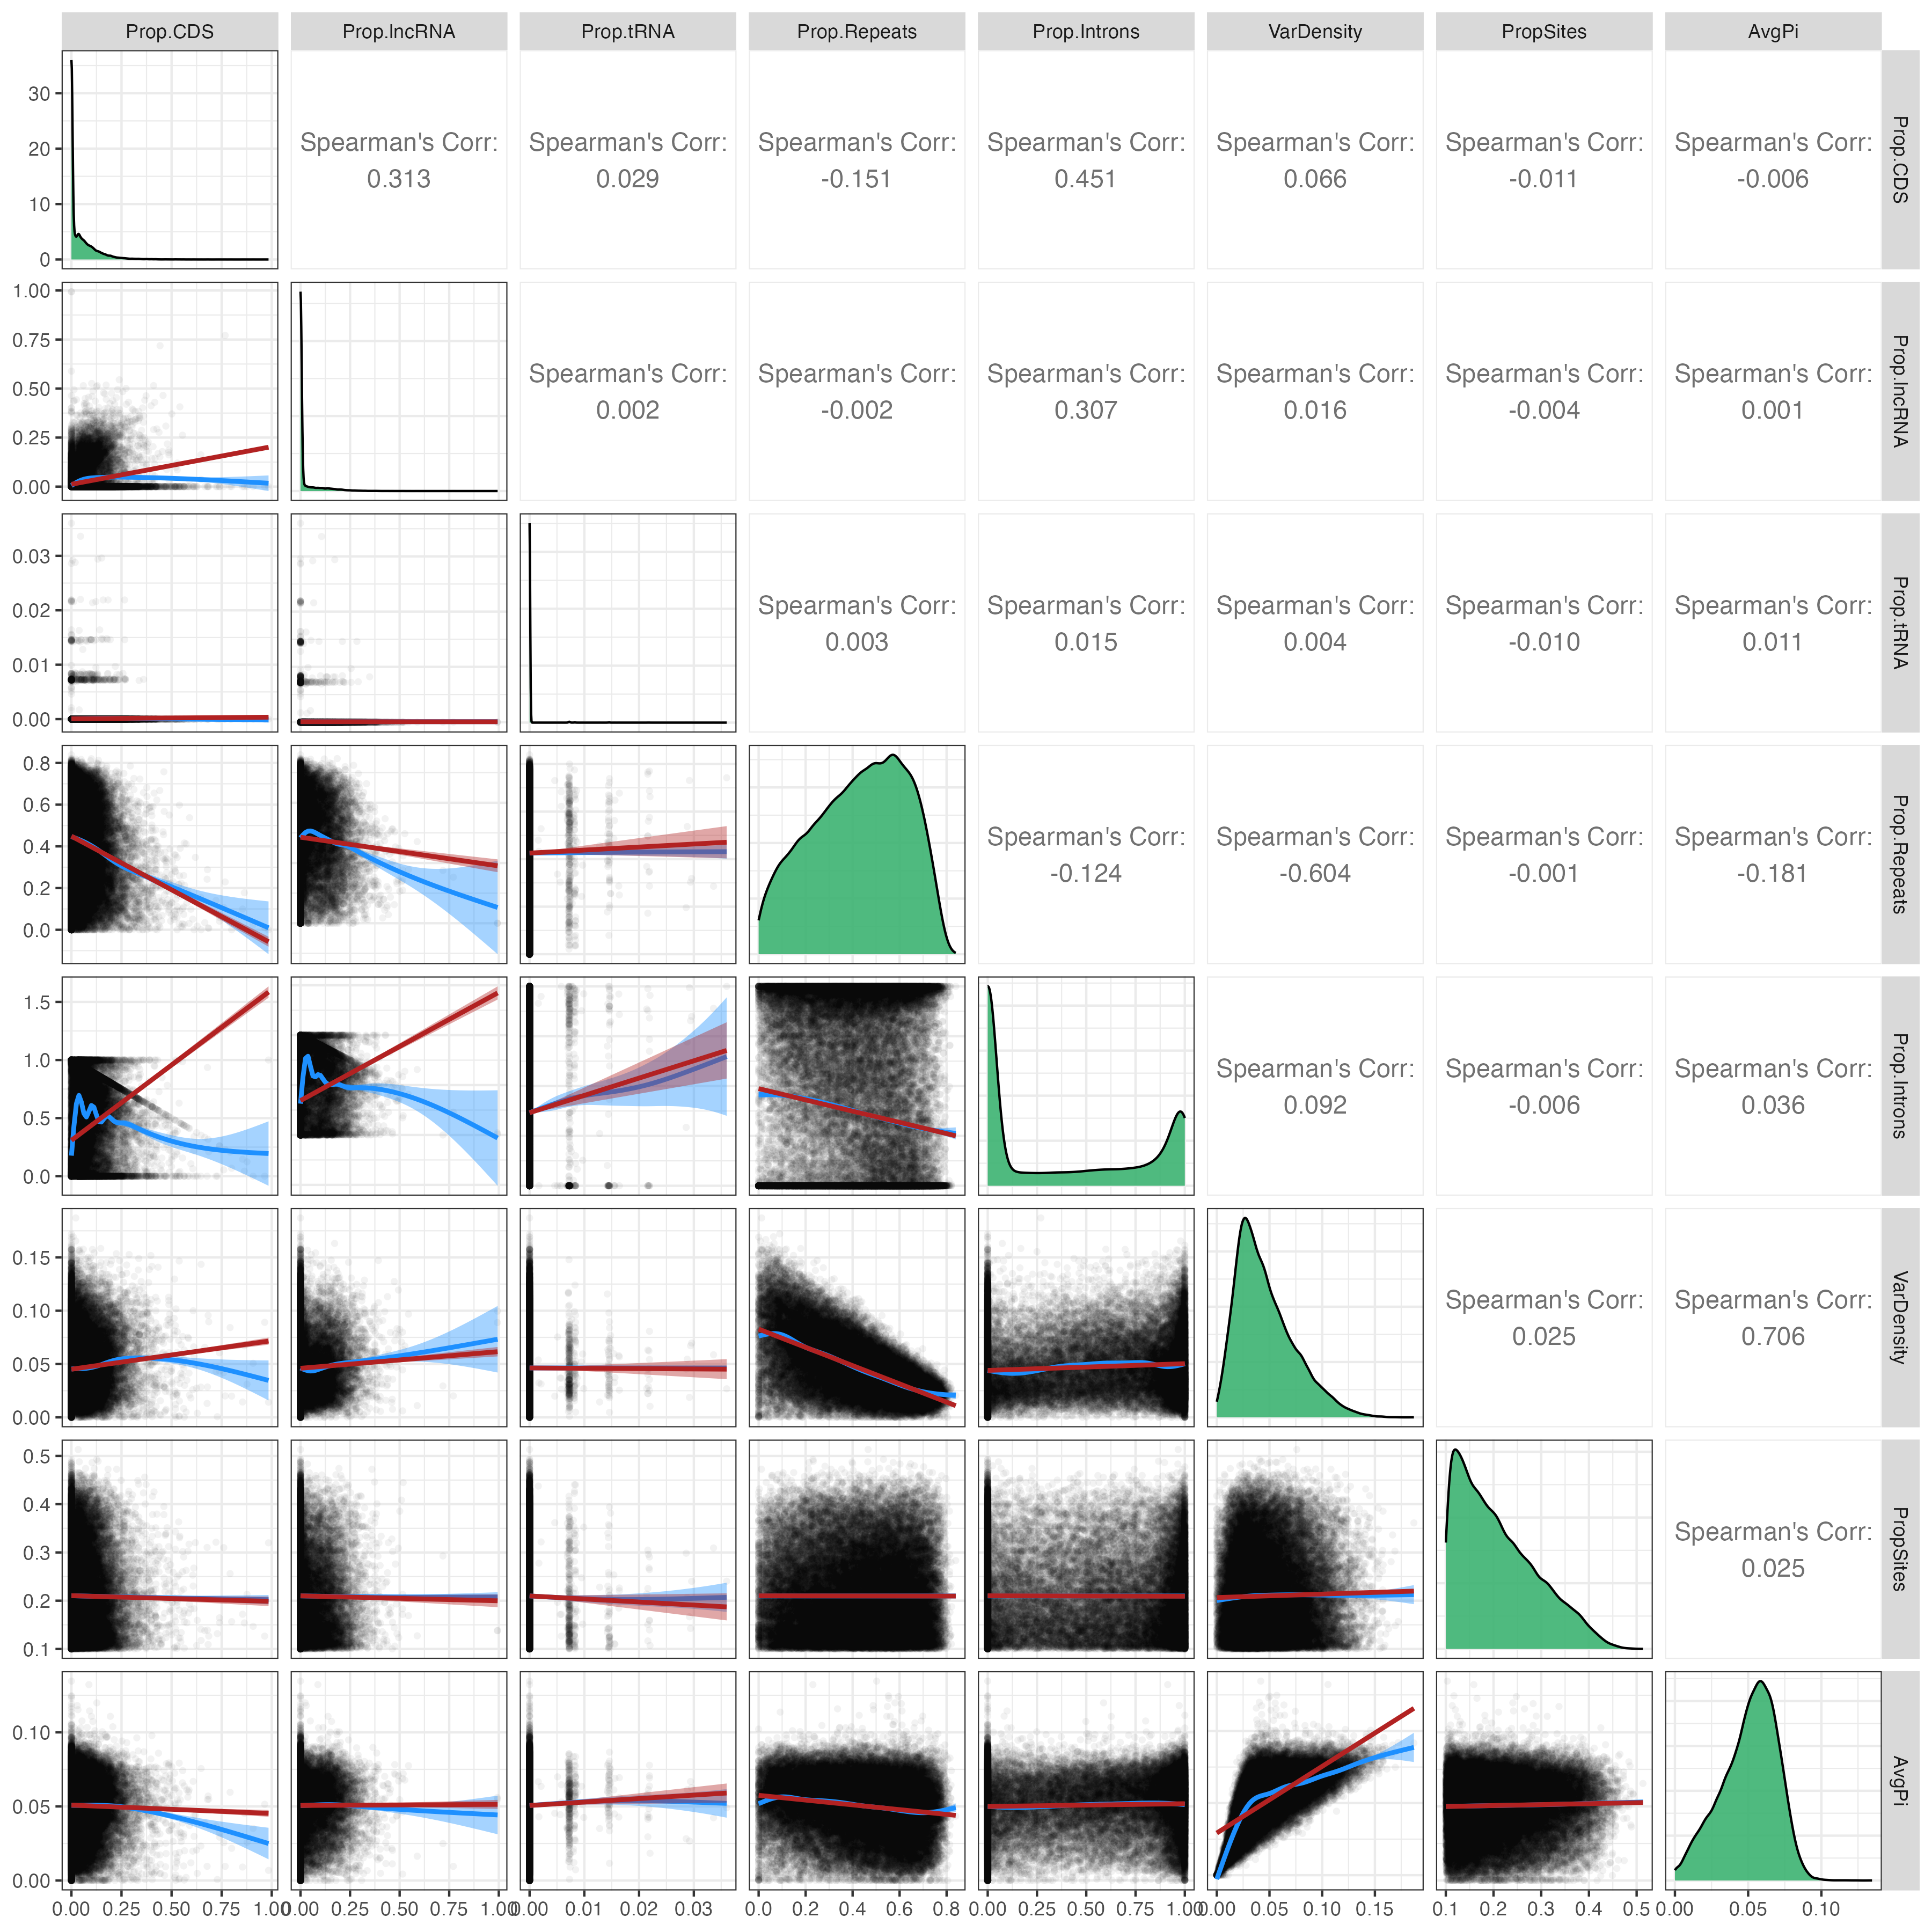
\includegraphics[width=1.0\textwidth]{figures/sups_pi_pairplot.png}
    \supfigurecaption{\textbf{Pairplot of genomic features and genetic variation
        in Oregon \balgla{}.}
        Diagonal shows the density histogram of the proportion of the genomics
        elements (e.g., CDS, lncRNA, tRNA, repeats, and introns), proportion of
        variant sites, proportion of callable sites post-filtering, and nucleotide
        diversity ($\pi$). All values computed across 10 kbp windows. Below
        the diagonal, plots show the correlation across all pairwise comparisons.
        Red and blue lines show the linear and Loess regression, respectively.
        Above the diagonal, panels show the Spearman's rank correlation
        coefficient ($\rho$) for the given pairwise comparison.}
    \label{fig:sup_pi_pairplot}
\end{figure}

% Theta_W Ne
\begin{figure}[ht]
    \centering
    \captionsetup{width=0.95\linewidth}
    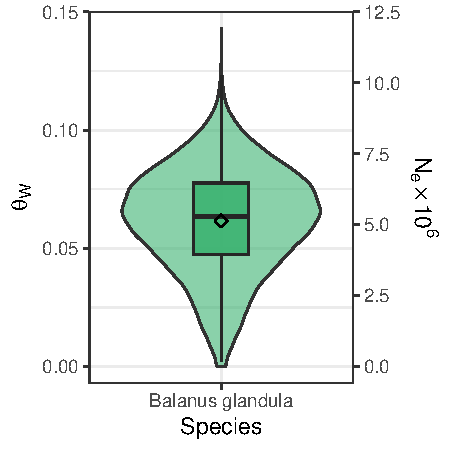
\includegraphics[width=0.7\textwidth]{figures/sups_theta_ne.pdf}
    \supfigurecaption{\textbf{Effective population (\Ne) size estimation
        of \balgla{} based on the Watterson's estimator ($\theta_\text{W}$).}
        Effective size of the population was calculated according to the
        relationship $\theta_\text{W}=4N_{e}\mu$, using a mutation rate per-base,
        per-generation ($\mu$) of $3\times10^{-9}$.
        This estimate yields a long-term \Ne{} of $\approx5.2\times10^{6}$ for
        this barnacle population.}
    \label{fig:sup_theta_ne}
\end{figure}

% msmc2 Ne
\begin{figure}[ht]
    \centering
    \captionsetup{width=0.95\linewidth}
    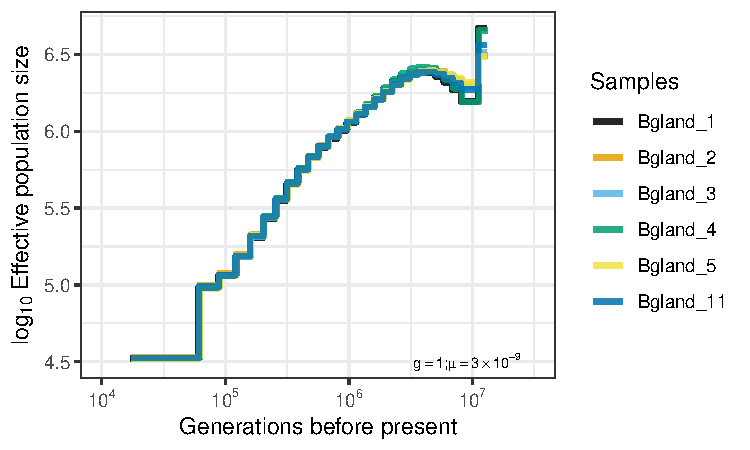
\includegraphics[width=0.9\textwidth]{figures/sups_msmc2_ne.pdf}
    \supfigurecaption{\textbf{Coalescent estimation of the effective
    population (\Ne) size estimation of \balgla{}.}
        Estimation of \Ne{} through time was done using the
        \textsc{msmc2} software, using a mutation rate per-base,
        per-generation ($\mu$) of $3\times10^{-9}$, and fixing the
        generation time ($g$) to 1.
        Each line represents the \Ne{} trajectory for each sample.
        Using just six diploid samples, and estimating only between pairs
        of unphased diploid genotypes within samples, we estimate the
        historical effective size of the population in the order of $10^{6}$
        individuals; however, we do not obtain enough resolution to resolve
        \Ne{} at recent ($<10^{5}$) time intervals.}
    \label{fig:sup_mcmc_ne}
\end{figure}

